\documentclass[12pt,letterpaper,noanswers]{exam}
\usepackage[usenames,dvipsnames,svgnames,table]{xcolor}
\usepackage[margin=0.9in]{geometry}
\renewcommand{\familydefault}{\sfdefault}
\usepackage{multicol}
\usepackage{wrapfig}
\pagestyle{head}
\definecolor{c03}{HTML}{FFDDDD}
\header{AM 22b Class 21}{}{Mar 19: Line integral}
\runningheadrule
\headrule
\usepackage{graphicx} % more modern
\usepackage{amsmath} 
\usepackage{amssymb} 
\usepackage{hyperref}
\usepackage{tcolorbox}
\usepackage[utf8]{inputenc}
\pagenumbering{arabic}

\usepackage[numbered,autolinebreaks,useliterate]{mcode}

\newcommand{\mb}[1]{\underline{#1}}

\begin{document}
 \pdfpageheight 11in 
  \pdfpagewidth 8.5in




% I need to review the torus trajectories...

\begin{itemize}
% \item There is a pre-class assignment (20 minutes of videos + a few WeBWorK exercises) due at 10am this Monday.  It is available on Canvas.
\itemsep0em
    \item Problem set 06 is due Thursday Mar 25th at 6pm.
  %  \item The Quiz 01 follow up assignment is due on Wednesday Mar 4th at midnight.
    \item Quiz 03 will be posted later today and will be available until 6pm ET on Sunday.
    \item There will be a skill check on Monday (C19, C20, C21).
\end{itemize}

\hrule
\vspace{0.2cm}

% partial derivatives, gradient
% local linearity, differential, directional deriv
% 2nd order partials + equations with partials

\noindent\textbf{Big picture}

On Wednesday we identified flow lines: curves that were perfectly aligned with the vectors of the vector field.  Today is focused on line integrals for vector fields: integrals that sum the component of a vector field along a curve through the vector field.  Line integrals can be used to compute the strength of rotation for a velocity vector field, or the work done by a force in a force vector field.

\vspace{0.2cm}
\hrule
\vspace{0.2cm}



\noindent\textbf{Skill Check C21 Practice}
\begin{questions}
\question Is the sign of the line integral for the pictured vector field and given curve to be positive, negative, or zero?

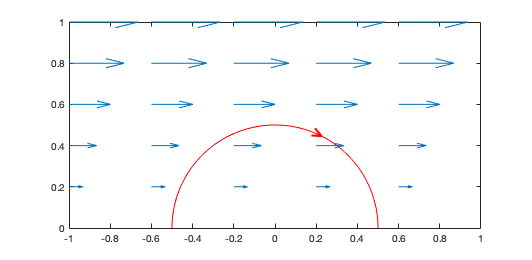
\includegraphics[width=4in]{img/C21lineintegral-p1.png}

\begin{oneparcheckboxes}
\choice positive
\choice negative
\choice zero
\end{oneparcheckboxes}
\end{questions}


\vspace{0.2cm}
\hrule
\vspace{0.2cm}

\noindent\textbf{Skill Check C21 Practice Solution}
\begin{questions}
\question The angle between the velocity vector direction and the vector field is less than $\pi/2$ at every point, so the dot product that contributes to the line integral will always be positive.  That means we are integrating a positive function, so the integral will be positive.
\end{questions}

\vspace{0.2cm}
\hrule
\vspace{0.2cm}

\noindent\textbf{Teams}
\begin{multicols}{2}

1.  students here

\end{multicols}

\eject
\vspace{0.2cm}
\hrule
\vspace{0.2cm}

\noindent\textbf{Line integrals: scalar function}.  \S 18.1  

\begin{tcolorbox}
\begin{itemize}
\itemsep0em
    \item A \textbf{line integral} is an integral where we integrate the value of a function along an oriented curve.
    \item A \textbf{line integral for a scalar field}, $f:\mathbb{R}^3 \rightarrow \mathbb{R}$, is given by \[\int_C f\ ds = \int_a^b f(\mb r(t)) \Vert \mb r'(t)\Vert dt\] with $\mb r(t), a\leq t\leq b$ a parameterization of $C$.
    \item A \textbf{scalar field} is a function with a single output.
\end{itemize}
\end{tcolorbox}


\href{https://upload.wikimedia.org/wikipedia/commons/4/42/Line_integral_of_scalar_field.gif}{\emph{click for illustrating gif}}


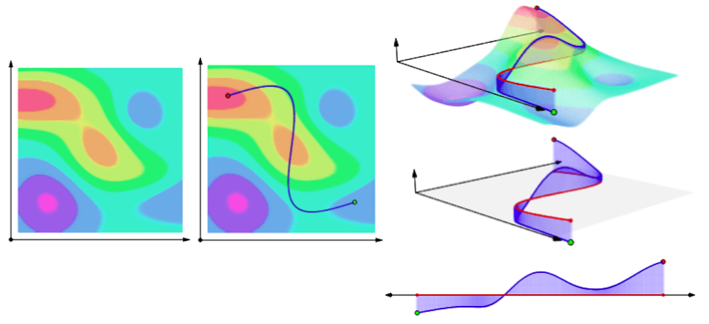
\includegraphics[width=\linewidth]{img/C25p1-18.png}
\url{https://upload.wikimedia.org/wikipedia/commons/4/42/Line_integral_of_scalar_field.gif}




\noindent\textbf{Example (mass).} 
Let $C$ be the shape of a wire parameterized by $x(t) = t, y(t) = t^2, 0\leq t\leq 1$.  Assume the wire has density $f(x,y) = k x^2$.  Rewrite the integral $\displaystyle\text{Mass} = \int_C f \ ds$ as an integral with respect to time.

\vspace{3in}

\vspace{0.2cm}
\hrule
\vspace{0.2cm}

\noindent\textbf{Line integral: vector field} \S 18.1
\begin{tcolorbox}
\begin{itemize}
\itemsep0em
    \item A \textbf{line integral for a vector field}, $\mb F:\mathbb{R}^3 \rightarrow \mathbb{R}^3$, along an oriented curve, $C$, is given by \[\int_C \mb F(\mb r)\cdot \mb T\ ds = \int_a^b \mb F(\mb r(t))\cdot \frac{d\mb r}{dt}\ dt\] where $\mb T$ is a unit vector in the direction tangent to $C$, and $\mb r(t)$ with $a\leq t\leq b$ is a parameterization of $C$. \href{https://upload.wikimedia.org/wikipedia/commons/b/b0/Line_integral_of_vector_field.gif}{\emph{click for illustrating gif}}
    \item Another notation for this is \[\int_C \mb F(\mb r)\cdot d\mb r = \int_a^b \mb F(\mb r(t)) \cdot \frac{d\mb r}{dt}dt\] with $\mb r(t), a\leq t\leq b$ a parameterization of $C$.
\end{itemize}



\tcblower

\begin{itemize}
\itemsep0em
    \item A line integral in a force vector field is used to compute the \textbf{work} done by a force to move an object (with mass or electric charge) along a path.

\item A \textbf{circulation} integral (a line integral where the curve $C$ is closed, denoted $\oint_C \mb F\cdot d\mb r$) is used to compute the circulation of a velocity vector field along a closed curve.  The circulation tells us about the net alignment of the vector field with the closed curve.

In the Kutta-Joukowski model of lift, circulation is an important component of modeling the lift force on an airplane wing.
\end{itemize}
\end{tcolorbox}

\noindent\textbf{Setting up a line integral}. 
Show that
\[\int_C \mb F(\mb r)\cdot \mb T\ ds = \int_a^b \mb F(\mb r(t))\cdot \frac{d\mb r}{dt}\ dt\] when the oriented curve $C$ is parameterized by $\mb r(t), a\leq t\leq b$. 
Recall that $\displaystyle\mb v = \frac{d\mb r}{dt}$, that $\displaystyle\mb T = \frac{\mb v}{\Vert\mb v\Vert},$ and that $\displaystyle ds = \Vert \mb v\Vert dt$.
\vspace{1in}


\noindent\textbf{Vector field vs scalar field}

Compare $\int_C f\ ds$ and $\int_C \mb F(\mb r)\cdot \mb T\ ds$.  $\mb F(\mb r)\cdot \mb T$ is a scalar.  What does it represent?

\hspace{-0.3in}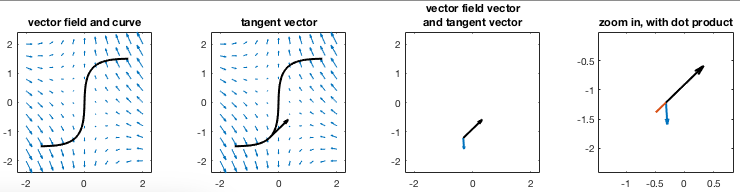
\includegraphics[width=0.8\linewidth]{img/C25p3-18.png}

\vspace{1in}


\noindent\textbf{Line integrals: identifying the sign} \S 18.1
\begin{tcolorbox}
\begin{itemize}
\itemsep0em
    \item Let $f(\mb r) = \mb F(\mb r)\cdot \mb T$.  If $f(\mb r)>0$ on $C$ then $\int_C f\ ds>0$.  If $f(\mb r)<0$ on $C$ then $\int_C f\ ds < 0$.  If $f(\mb r) = 0$ on $C$ then $\int_C f\ ds = 0$.  In these cases, the sign of the line integral can be identified without further reasoning.
    \item Sometimes $\mb F(\mb r)\cdot \mb T$ is symmetric, with positive values on one part of a curve that are exactly balanced by corresponding negative values on another part of the curve, so that $\int_C f\ ds = 0$.
    \item Other times, $\mb F(\mb r)\cdot \mb T$ is not symmetric, and it is possible to identify whether the negative contribution to the line integral dominates the positive contribution.  In such cases, identifying the sign of the line integral may be possible.
\end{itemize}
\end{tcolorbox}

\noindent\textbf{Sign of a line integral}.
The line integral is $\displaystyle\int_C \mb F(\mb r)\cdot \mb T\ ds$.  Identify the sign of 

$\displaystyle\int_{C_1} \mb F(\mb r)\cdot \mb T\ ds$,

$\displaystyle\int_{C_2} \mb F(\mb r)\cdot \mb T\ ds$,

$\displaystyle\int_{C_3} \mb F(\mb r)\cdot \mb T\ ds$,

$\displaystyle\int_{C_4} \mb F(\mb r)\cdot \mb T\ ds$ using the image below.


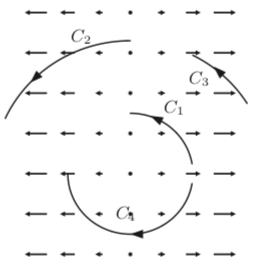
\includegraphics[width=2in]{img/C25p2-18.png}

\textbf{Extra}: For $C_1, C_2, C_4$, put the line integrals in order from least to greatest.


\vfill
\eject
\noindent\textbf{Circulation}.  A circulation integral is the line integral about a closed curve.  Let $C$ be a circle centered at the origin and oriented clockwise.  Identify the sign of the circulation around $C$ for each of the vector fields below.  

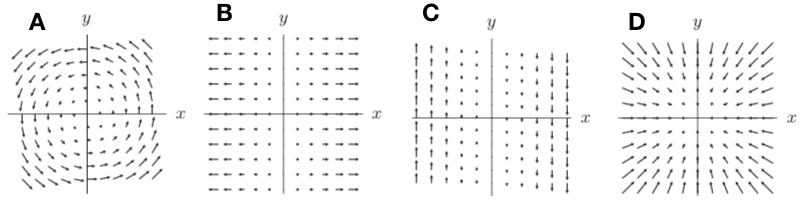
\includegraphics[width=\linewidth]{img/C25p4-18.png}
\vfill



\noindent\textbf{Line integrals}.  Pair the line integrals that are equal based on the diagrams below.

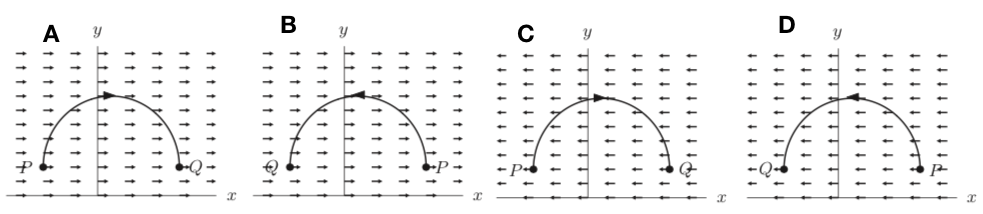
\includegraphics[width=\linewidth]{img/C25p5-18.png}

\vfill

%\eject
\noindent\textbf{Work done by a vector field}.  The work done by a force field is given by $\int_C \mb F\cdot d\mb r$.  Let $\mb F = y\mb i$ be a force field.  An object moves along a straight line joining $(1,1)$ to $(1,-1)$.  Find the sign of the work done by the force field. % \emph{pollQ}


\textbf{Extra:} Give paths for which the other cases would occur.  Give vector fields for which the other cases would occur.

\vfill

\eject

% \noindent\textbf{Gradient field}.  Let $\mb F = \mb \nabla f$ for some function $f$, so $\mb F$ is a gradient field.  Consider $\int_C \mb\nabla f\cdot d\mb r$.  Recall $\int_C \mb \nabla f \cdot d\mb r = \int_C \mb \nabla f\cdot \mb T\ ds$.  A Riemann sum approximation for the line integral is $\sum \mb\nabla f(\mb r_i)\cdot \mb T \Delta s_i$.  Which of the following statements hold?

% \begin{enumerate}
%     \item On a segment $\Delta s_i$ where $C$ crosses a level curve of $f$ in a direction where $f$ is increasing, there is a positive contribution to the Riemann sum.
%     \item On a segment $\Delta s_i$ where $f$ is positive there is a positive contribution to the Riemann sum.
%     \item On a segment $\Delta s_i$ where $C$ is tangent to a level curve of $f$ there is a positive contribution to the Riemann sum.
% \end{enumerate}

% \vfill

\noindent\textbf{Problem}.  Let $C$ be the line segment from the origin to $(1,1,1)$.  Let $\mb F = ay\mb i -ax\mb j + (b-1)\mb k$.  Give conditions on $a$ and $b$ so that the line integral $\int_C \mb F\cdot d\mb r$ is positive.
\vfill


\vspace{0.2cm}
\hrule
\vspace{0.2cm}




\end{document}